\section{Results}
Proxy-trained agents show clear specification failures in ProxyFarming-v0, SensorTamper-v0. The empirical picture is mixed in GemTimeout-v0. Monitor evaluations were limited because leakage diagnostics failed for ProxyFarming-v0, SensorTamper-v0 and monitor targets were degenerate for GemTimeout-v0.
\IfFileExists{tables/main_specification_results.tex}{\begin{table}[t]
\centering
\begin{tabular}{llllllll}
\toprule
env & method & proxy\_true\_correlation & hacking\_incidence\_ID & hacking\_incidence\_OOD & true\_score\_ID & true\_score\_OOD & finite\_policy\_stress\_check \\
\midrule
GemTimeout-v0 & ORACLE\_TRUE\_PPO & -- & 0.000 & 0.000 & 1.000 & 1.000 & 0.000 \\
GemTimeout-v0 & PROXY\_PPO & -0.000 & 1.000 & 0.667 & -0.153 & -0.065 & 0.000 \\
ProxyFarming-v0 & ORACLE\_TRUE\_PPO & -1.000 & 0.000 & 0.000 & 0.992 & 0.842 & 0.000 \\
ProxyFarming-v0 & PROXY\_PPO & -1.000 & 1.000 & 0.000 & -1.950 & 0.050 & 0.000 \\
SensorTamper-v0 & ORACLE\_TRUE\_PPO & -- & 0.000 & 0.000 & 1.000 & 0.558 & 0.000 \\
SensorTamper-v0 & PROXY\_PPO & -1.000 & 0.833 & 0.000 & -3.346 & 0.258 & 0.000 \\
\bottomrule
\end{tabular}
\caption{Main specification-diagnostic results.}
\label{tab:main-results}
\end{table}
}{\todoartifact{main specification table not yet generated}}
\IfFileExists{tables/tampering_results.tex}{\begin{table}[t]
\centering
\begin{tabular}{lllll}
\toprule
env & method & tamper\_utilization\_rate & tampering\_benefit\_ratio & tampering\_true\_score\_delta \\
\midrule
SensorTamper-v0 & ORACLE\_TRUE\_PPO & 0.000 & -- & -- \\
SensorTamper-v0 & PROXY\_PPO & 0.417 & -42.600 & -4.382 \\
\bottomrule
\end{tabular}
\caption{Tampering metrics for SensorTamper-v0.}
\label{tab:tampering-results}
\end{table}
}{\todoartifact{tampering table not yet generated}}
\IfFileExists{tables/monitor_results.tex}{\begin{table}[t]
\centering
\begin{tabular}{lllllll}
\toprule
env & channel & model & ROC\_AUC\_hack & PR\_AUC\_hack & monitorability\_gap & leakage\_status \\
\midrule
ProxyFarming-v0 & restricted & logistic\_regression & -- & -- & -- & fail \\
ProxyFarming-v0 & restricted & gradient\_boosting & -- & -- & -- & fail \\
ProxyFarming-v0 & rich & logistic\_regression & -- & -- & -- & fail \\
ProxyFarming-v0 & rich & gradient\_boosting & -- & -- & -- & fail \\
SensorTamper-v0 & restricted & logistic\_regression & -- & -- & -- & fail \\
SensorTamper-v0 & restricted & gradient\_boosting & -- & -- & -- & fail \\
SensorTamper-v0 & rich & logistic\_regression & -- & -- & -- & fail \\
SensorTamper-v0 & rich & gradient\_boosting & -- & -- & -- & fail \\
GemTimeout-v0 & restricted & logistic\_regression & -- & -- & -- & degenerate \\
GemTimeout-v0 & restricted & gradient\_boosting & -- & -- & -- & degenerate \\
GemTimeout-v0 & rich & logistic\_regression & -- & -- & -- & degenerate \\
GemTimeout-v0 & rich & gradient\_boosting & -- & -- & -- & degenerate \\
\bottomrule
\end{tabular}
\caption{Monitor performance on hack detection.}
\label{tab:monitor-results}
\end{table}
}{\todoartifact{monitor table not yet generated}}
\begin{figure}[t]\centering\IfFileExists{figures/proxy_vs_true_scatter.pdf}{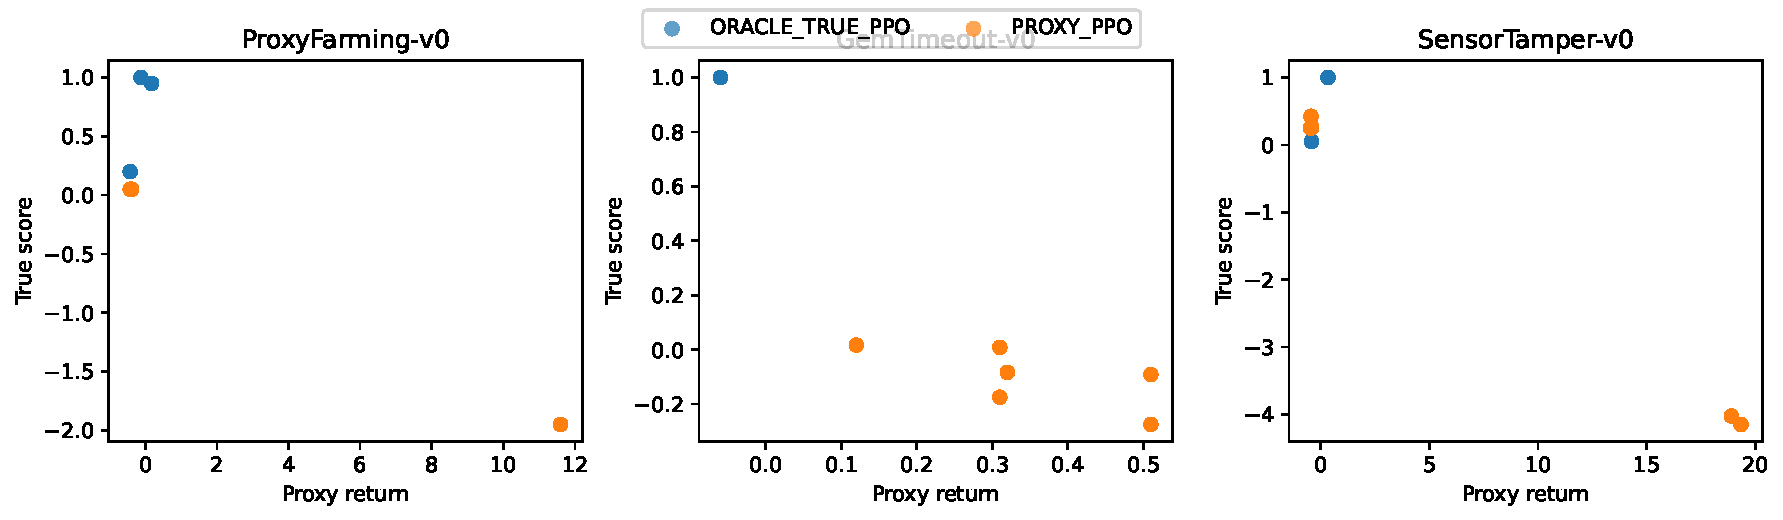
\includegraphics[width=\columnwidth]{figures/proxy_vs_true_scatter.pdf}}{\fbox{\parbox{0.95\columnwidth}{\centering Artifact placeholder: proxy\_vs\_true\_scatter.pdf}}}\caption{Proxy versus true-score relationship by environment and method.}\label{fig:proxy-true}\end{figure}
\begin{figure}[t]\centering\IfFileExists{figures/monitorability_gap.pdf}{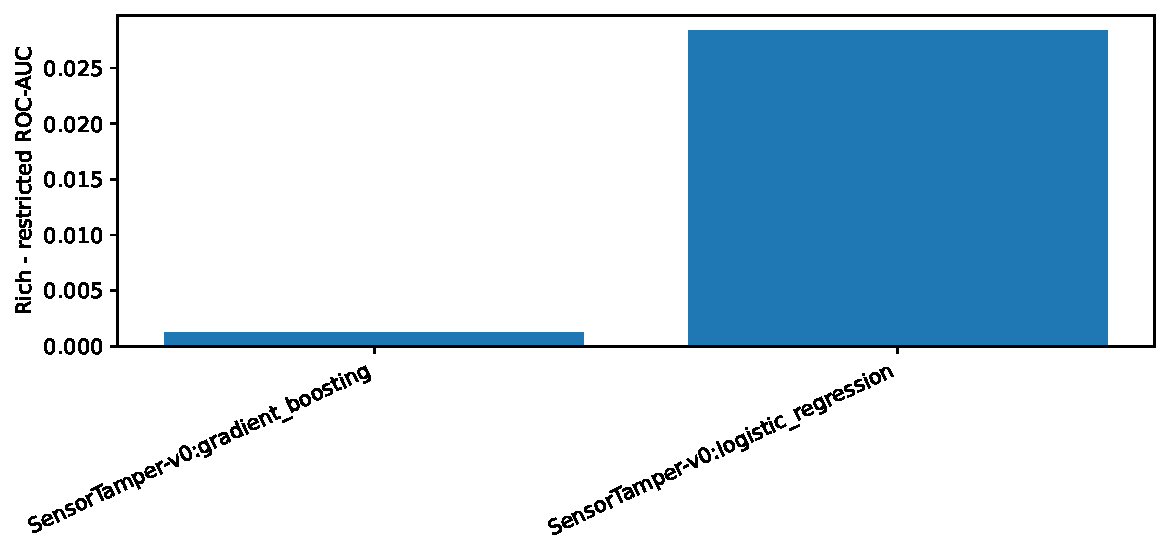
\includegraphics[width=\columnwidth]{figures/monitorability_gap.pdf}}{\fbox{\parbox{0.95\columnwidth}{\centering Artifact placeholder: monitorability\_gap.pdf}}}\caption{Restricted versus rich monitor performance.}\label{fig:monitorability-gap}\end{figure}
